\chapter{Versuchsdurchführung}

In der Durchführung werden einige in der Vorbereitung diskutierten Eigenschaften 
dreier Materialien untersucht. Diese wurden im letzten Abschnitt der Vorbereitung
diskutiert. 

\section{Messungen an der Graphitprobe}

Zunächst platziert man die Probe auf dem Halter und legt diesen in das Mikroskop. 
Eine grobe Annäherung an die Messspitze erfolgt per Hand. Beobachtet durch eine
Lupe über dem Aufbau kann mit den Piezoelementen die Spitze genauer an die Probe
herangeführt werden. Im letzten Schritt wird die Annäherung automatisch 
ausgeführt, bis der vorgegebene Tunnelstrom erreicht wurde. Bei der Graphitprobe
darf der Tunnelstrom einen Wert von $\SI{1}{nA}$ nicht überschreiten. Die 
Tunnelspannung wird auf $\SI{50}{mV}$ gesetzt.\par

\subsection{Topographie}

Mit diesen Einstellungen können erste Aufnahmen der Oberfläche gemacht werden.
Zuerst wird hierbei ein großer Bereich der Oberfläche gemessen. Aus diesem
Bild wird dann ein möglichst homogener Bereich zur näheren Messung ausgewählt.
Die Neigung der Probe zur Spitze wird parallel in einem Linienprofil gemessen.
Dies ermöglicht einen Ausgleich, um Verzerrungen im Bild vorzubeugen.
So entsteht schließlich ein Bild der Oberfläche mit atomarer Auflösung.
\begin{figure}[H]
    \centering
    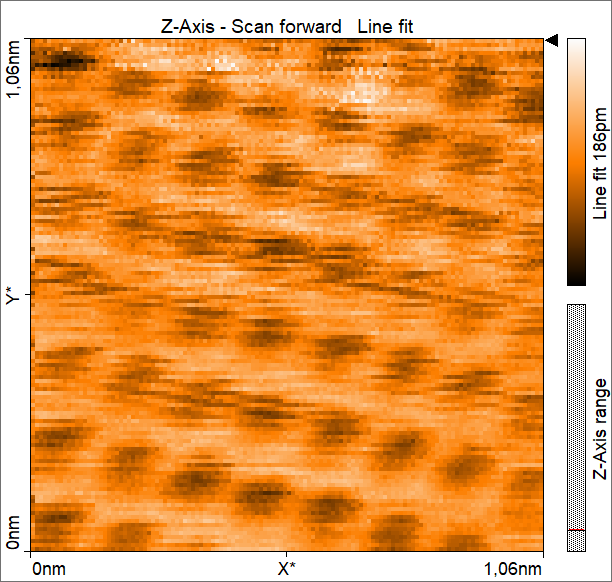
\includegraphics[width=0.5\textwidth]{Mess/graphit_oberfl.png}
    \caption{Topographie von Graphit}
    \label{topo_graphit}
\end{figure}
Abbildung \ref{topo_graphit} zeigt die Oberfläche im atomaren Bereich.
Um gute Bilder in dieser Auflösung zu erreichen ist eine gute Spitze, eine
homogene Oberfläche und viel Geschick nötig. 
\begin{figure}[h]
    \centering
    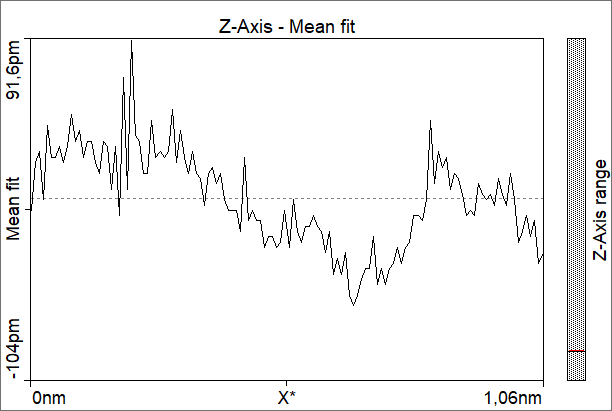
\includegraphics[width=0.6\textwidth]{Mess/graphit_linienprofil.png}
    \caption{Linienprofil der gemessenen Graphitoberfläche}
    \label{graprof}
\end{figure}
In Abbildung \ref{graprof} ist das zur gemessenen Oberfläche gehörige Linienprofil
in x-Richtung abgebildet. 
Die zu erkennende Inhomogenität der Oberfläche könnte ein Grund für die 
geringe Auflösung der Oberflächenmessung sein. Auch könnte eine mangelhafte
Spitze ein schlechtes Ergebnis verursachen.

\subsection{Spektroskopie}
\paragraph{Strom-Spannungs-Kennlinie}
Im nächsten Schritt soll die Strom-Spannungs-Kennlinie aufgenommen werden. 
%\begin{figure}
%    \centering
%    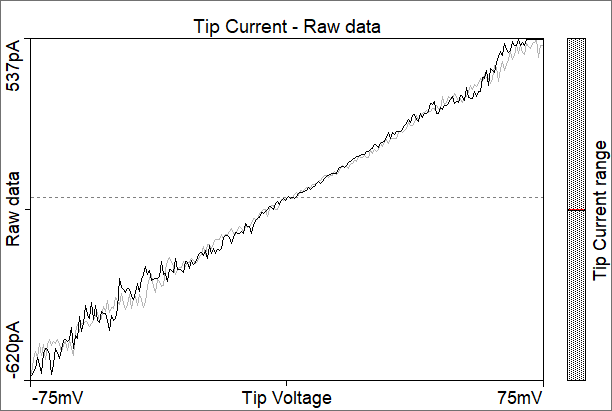
\includegraphics[width=0.7\textwidth]{Mess/graphit_ui.png}
%    \caption{Strom-Spannungs-Kennlinie von Graphit}
%    \label{graui}
%\end{figure}
\begin{figure}[h]
  \centering
  \begin{tikzpicture}
    \begin{axis}[
            xlabel={Spannung [mV]},
            ylabel={Tunnelstrom [pA]},
      %xmin=25,xmax=200,
      /pgf/number format/1000 sep={},
      legend pos=north west
    ]
    \addplot[ 
      color = black,
      mark  = none,
      thick
    ] table [
				%x=verz,y=int,
        x expr=\thisrowno{0}*10^3,
        y expr=\thisrowno{1}*10^12
			]
    {Mess/strom_spannung_graphit.plt};
         \addlegendentry{Messwerte}
       \end{axis}
  \end{tikzpicture} 
  \caption{Strom-Spannungskurve von Graphit}
  \label{graphui}
\end{figure}
Das Ergebnis der Messung ist in Abbildung \ref{graphui} zu sehen. Die Spannung der 
Spitze wird von $\SI{-75}{mV}$ bis $\SI{75}{mV}$ variiert. Hier könnte die Spannung
noch höher gewählt werden, da der maximale Tunnelstrom von $\SI{1}{nA}$ noch nicht
erreicht wurde. Dies hätte das Rauschen der Kurve weiter reduziert.
Der erwartete lineare Verlauf,wie in Kapitel \ref{spek} diskutiert,
ist dennoch eindeutig erkennbar.

\paragraph{Strom-Abstands-Kennlinie}
Im zweiten Teil der Spektroskopie soll die exponentielle Zunahme des Tunnelstroms
mit dem Abstand, wie auch im Kapitel \ref{spek} hergeleitet, experimentell 
überprüft werden. Hierzu wird die Entfernung von Probe und Spitze bei konstanter
Spannung variiert. 
%\begin{figure}
%    \centering
%    \includegraphics[width=0.7\textwidth]{Mess/graphit_di.png}
%    \caption{Strom-Abstands-Kennlinie von Graphit}
%    \label{graphdi}
%\end{figure}
\begin{figure}[h]
  \centering
  \begin{tikzpicture}
    \begin{axis}[
            xlabel={Abstand [nm]},
            ylabel={Tunnelstrom [nA]},
      %xmin=25,xmax=200,
      /pgf/number format/1000 sep={},
      ymode=log,
      legend pos=north west,
      ymin=10e-4
    ]
    \addplot[ 
      color = black,
      mark  = none,
      thick
    ] table [
				%x=verz,y=int,
        x expr=\thisrowno{0}*10^9,
        y expr=\thisrowno{1}*10^9
			]
    {Mess/strom_abstand_graphit.plt};
		\addlegendentry{Messwerte}
    \end{axis}
  \end{tikzpicture} 
  \caption{Strom-Abstands-Kennlinie von Graphit logarithmisch aufgetragen}
  \label{graphdi}
\end{figure}
Das Ergebnis ist in Abbildung \ref{graphdi} zu sehen. Die y-Achse ist hierbei
logarithmisch aufgetragen, um den exponentiellen Zusammenhang leichter ersichtlich
zu machen. Die x-Werte, also der Abstand, werden vom Messprogramm nicht richtig
ausgegeben. Die Größe des gemessenen Intervalls von ca. $\SI{1}{nm}$ stimmt, 
jedoch ist der Ursprung der Achse nicht die Oberfläche des Materials.
Bei dieser Messung ist leider ein starkes Rauschen zu erkennen. Dies ist in 
Anbetracht der ebenso verrauschten Topographie jedoch kaum verwunderlich.
Der exponentielle Zusammenhang ist trotzdem zu erkennen.

\subsection{Vermessung des Graphitgitters}
Anhand der Oberflächenmessung des Graphits kann noch eine Vermessung dieser
versucht werden.
\begin{figure}[h]
    \begin{subfigure}[c]{0.45\textwidth}
        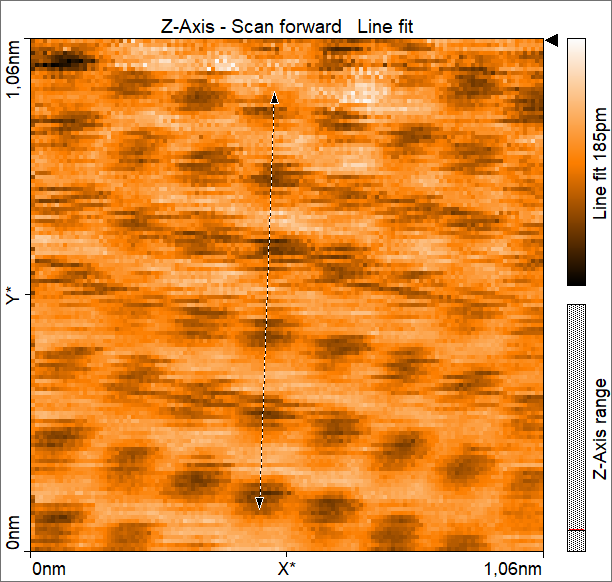
\includegraphics[width=\textwidth]{Mess/graphit_gitterkonst.png}
    \end{subfigure}
    \begin{subfigure}[c]{0.45\textwidth}
        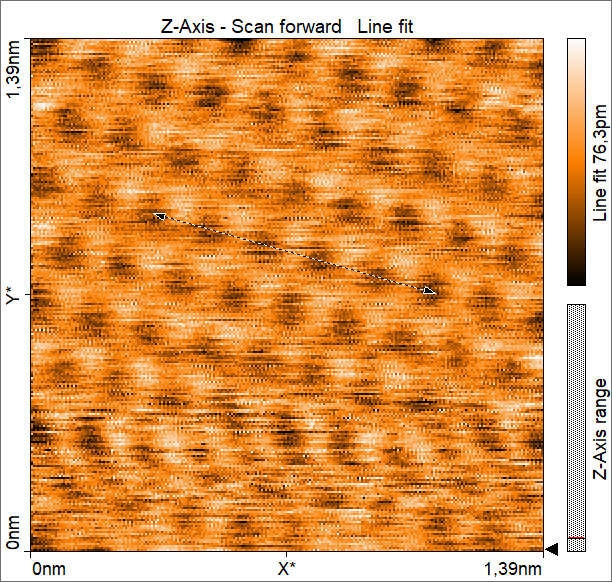
\includegraphics[width=\textwidth]{Mess/graphit_gitterkonst2.png}
    \end{subfigure}
    \caption{Bestimmung der Gitterkonstante von Graphit}
    \label{graphgit}
\end{figure}
Hierzu wurde mithilfe des Werkzeuge des Messprogramms der Abstand von sechs
Atomen gemessen, zu sehen in Abbildung \ref{graphgit}. Der gemessene Abstand
beträgt $\SI{919}{pm}$. Im $60^\circ$ Winkel dazu wird diese Messung wiederholt,
hier werden $\SI{732}{pm}$ gemessen. Auf einem zweiten Bild werden die Werte
$\SI{897}{nm}$ und $\SI{798}{nm}$ gemessen. Nimmt man den Mittelwert und teilt
diesen durch die fünf Atomabstände, so errechnet sich ein Wert von $\SI{167}{pm}$
für den Abstand zweier Atome.
Dies weicht vom Literaturwert $\SI{245}{pm}$ stark ab. Dieser Messfehler kann 
wiederum bei der inhomogene Oberfläche und der Spitze vermutet werden.\par
Weiter lässt sich der Winkel zwischen den Atomlagen messen, wie in Abbildung
\ref{graphwinkel} zu sehen. 
\begin{figure}[h]
    \centering
    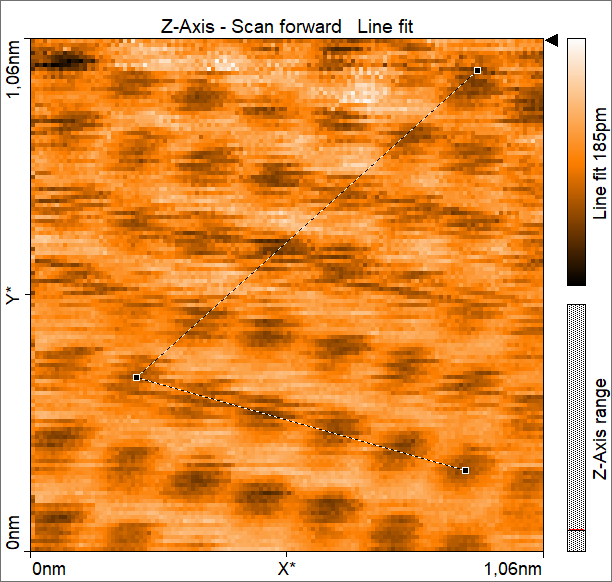
\includegraphics[width=0.5\textwidth]{Mess/graphit_winkel.png}
    \caption{Winkelmessung im Graphit}
    \label{graphwinkel}
\end{figure}
Hierbei wird ein Winkel von $57,5^\circ$ gemessen. Diese kleine Abweichung
kann durch die Inhomogenität der Oberfläche erklärt werden.

\subsection{3D-Darstellung des Gitters}
Im letzten Schritt sollen mithilfe der WSxM Software einige 3D-Bilder der 
Oberfläche erstellt werden. Die Ergebnisse sind in Abbildung \ref{graphit3d}
zu sehen.
\begin{figure}[h]
    \begin{subfigure}[c]{0.5\textwidth}
        \centering
        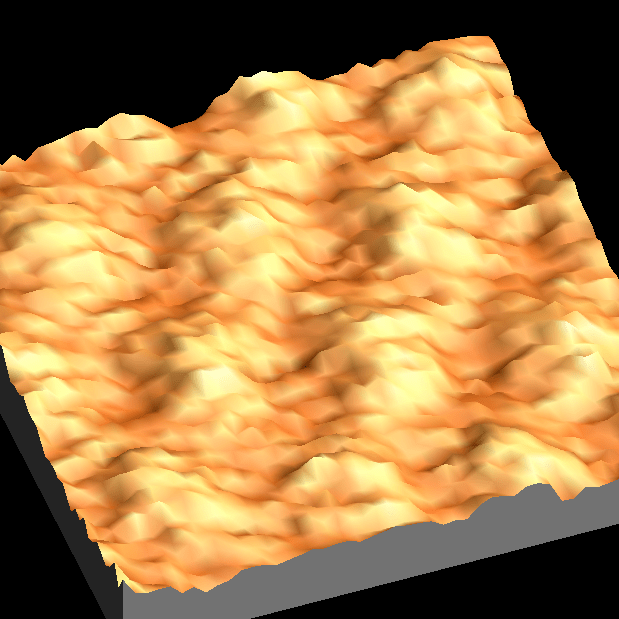
\includegraphics[width=\textwidth]{Mess/graphit3d.bmp}
    \end{subfigure}
    \begin{subfigure}[c]{0.5\textwidth}
        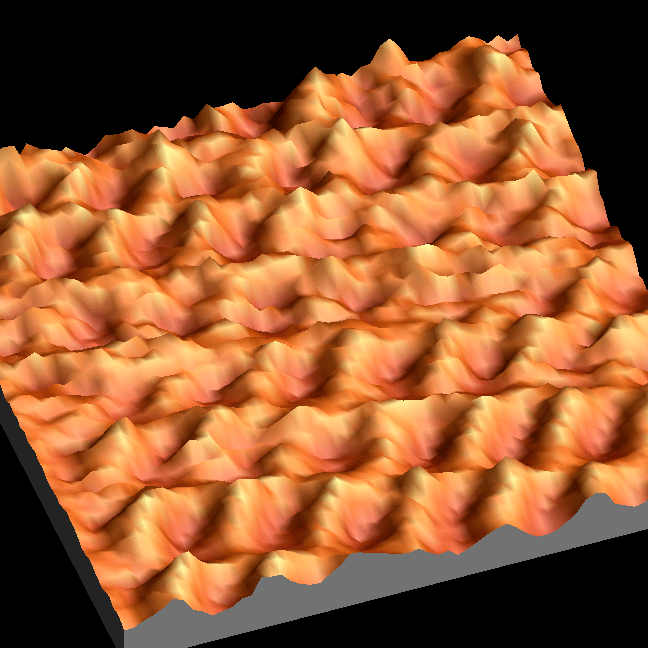
\includegraphics[width=\textwidth]{Mess/graphit3d2.bmp}
    \end{subfigure}
    \caption{3D-Darstellung der Messdaten mithilfe von WSxM}
    \label{graphit3d}
\end{figure}

